\documentclass[]{article}

% Imported Packages
%------------------------------------------------------------------------------
\usepackage{amssymb}
\usepackage{amstext}
\usepackage{amsthm}
\usepackage{amsmath}
\usepackage{float}
\usepackage{enumerate}
\usepackage{fancyhdr}
\usepackage[margin=1in]{geometry}
\usepackage{graphicx}
\usepackage{extarrows}
\usepackage{setspace}
%------------------------------------------------------------------------------

% Header and Footer
%------------------------------------------------------------------------------
\pagestyle{plain}  
\renewcommand\headrulewidth{0.4pt}                                      
\renewcommand\footrulewidth{0.4pt}                                    
%------------------------------------------------------------------------------

% Title Details
%------------------------------------------------------------------------------
\title{SFWR ENG 3A04\\Deliverable \#2\\High-Level System Design}
\author{Jonathan Yu\\Samuel Jackson\\Bill Chen\\Fiona Hu\\Nikita Jagora}
\date{}                               
%------------------------------------------------------------------------------

% Document
%------------------------------------------------------------------------------
\begin{document}

\maketitle	

\section{Introduction}
\label{sec:introduction}

\subsection{Purpose}
\label{sec:purpose}

The purpose of this document is to describe the software architecture of the WhoDatDog mobile application. This document describes the hierarchy and structure of the system's components in terms of its' classes, by defining both each class of the system and the interractions between these classes. This document is intended for use by software design and system support personnel.

\subsection{System Description}
\label{sec:sysdescription}

The WhoDatDog system is a mobile application developed for mobile devices running a Google Android operating system of version 8.4.2 or higher. This system's primary function is to enable a user to identify the breed of a dog they may find in their immediate, physical environement. Additionally, the system enables users to search for locations where they may purchase or adopt a dog in their vicinity, i.e. pet stores, dog pounds, etc., and to create posts on the Twitter social network, to describe to other users a dog they have identified and the geographic location where they have seen it.\\\\In order to accomplish these functions, the WhoDatDog software system employs a hierarchial system architecture which includes user interfaces at the top level, system controllers at the bottom level, and system memory at the lower level. In particular, the system's memory contains three so-called "expert" systems which are used for dog breed identification, and the system also uses external systems in the form of Twitter and Google Maps plugins.

\subsection{Overview}
\label{sec:overview}

The contents of this document are organized into 6 sections, including Section 1, the introduction. Sections 2-5 which describe and define the software structure of the system in a different aspect.\\Section 2 contains use case diagrams of the system, which describe the external actors (i.e. users, etc.) and internal system software classes and interactions needed for the system to perform a particular functional system requirements.\\Section 3c contains an analysis class diagram, which identifies the controller, storage entity, and user/system interface boundary classes in the system and graphically displays how these classes are interconnected.\\Section 4 contains descriptions of the system architecture design. For both the entire system and all subsystems, this section describes the architecture design used and provides a justification of the design's use and a graphical diagram of the design.\\Section 5 of the document contains class responsibility collaboration (CRC) cards for all of the classes used in the system. Each card contains the name of the class it describes, and a brief description of the class's own responsibilities and the other classes it collaborates with.\\Though it does not describe the system, Section 5 states the division of labor among the authors of this document.

\section{Use Case Diagram}
\label{sec:use_case_diagram}
% Begin Section
\begin{figure}[H]
	\centering
	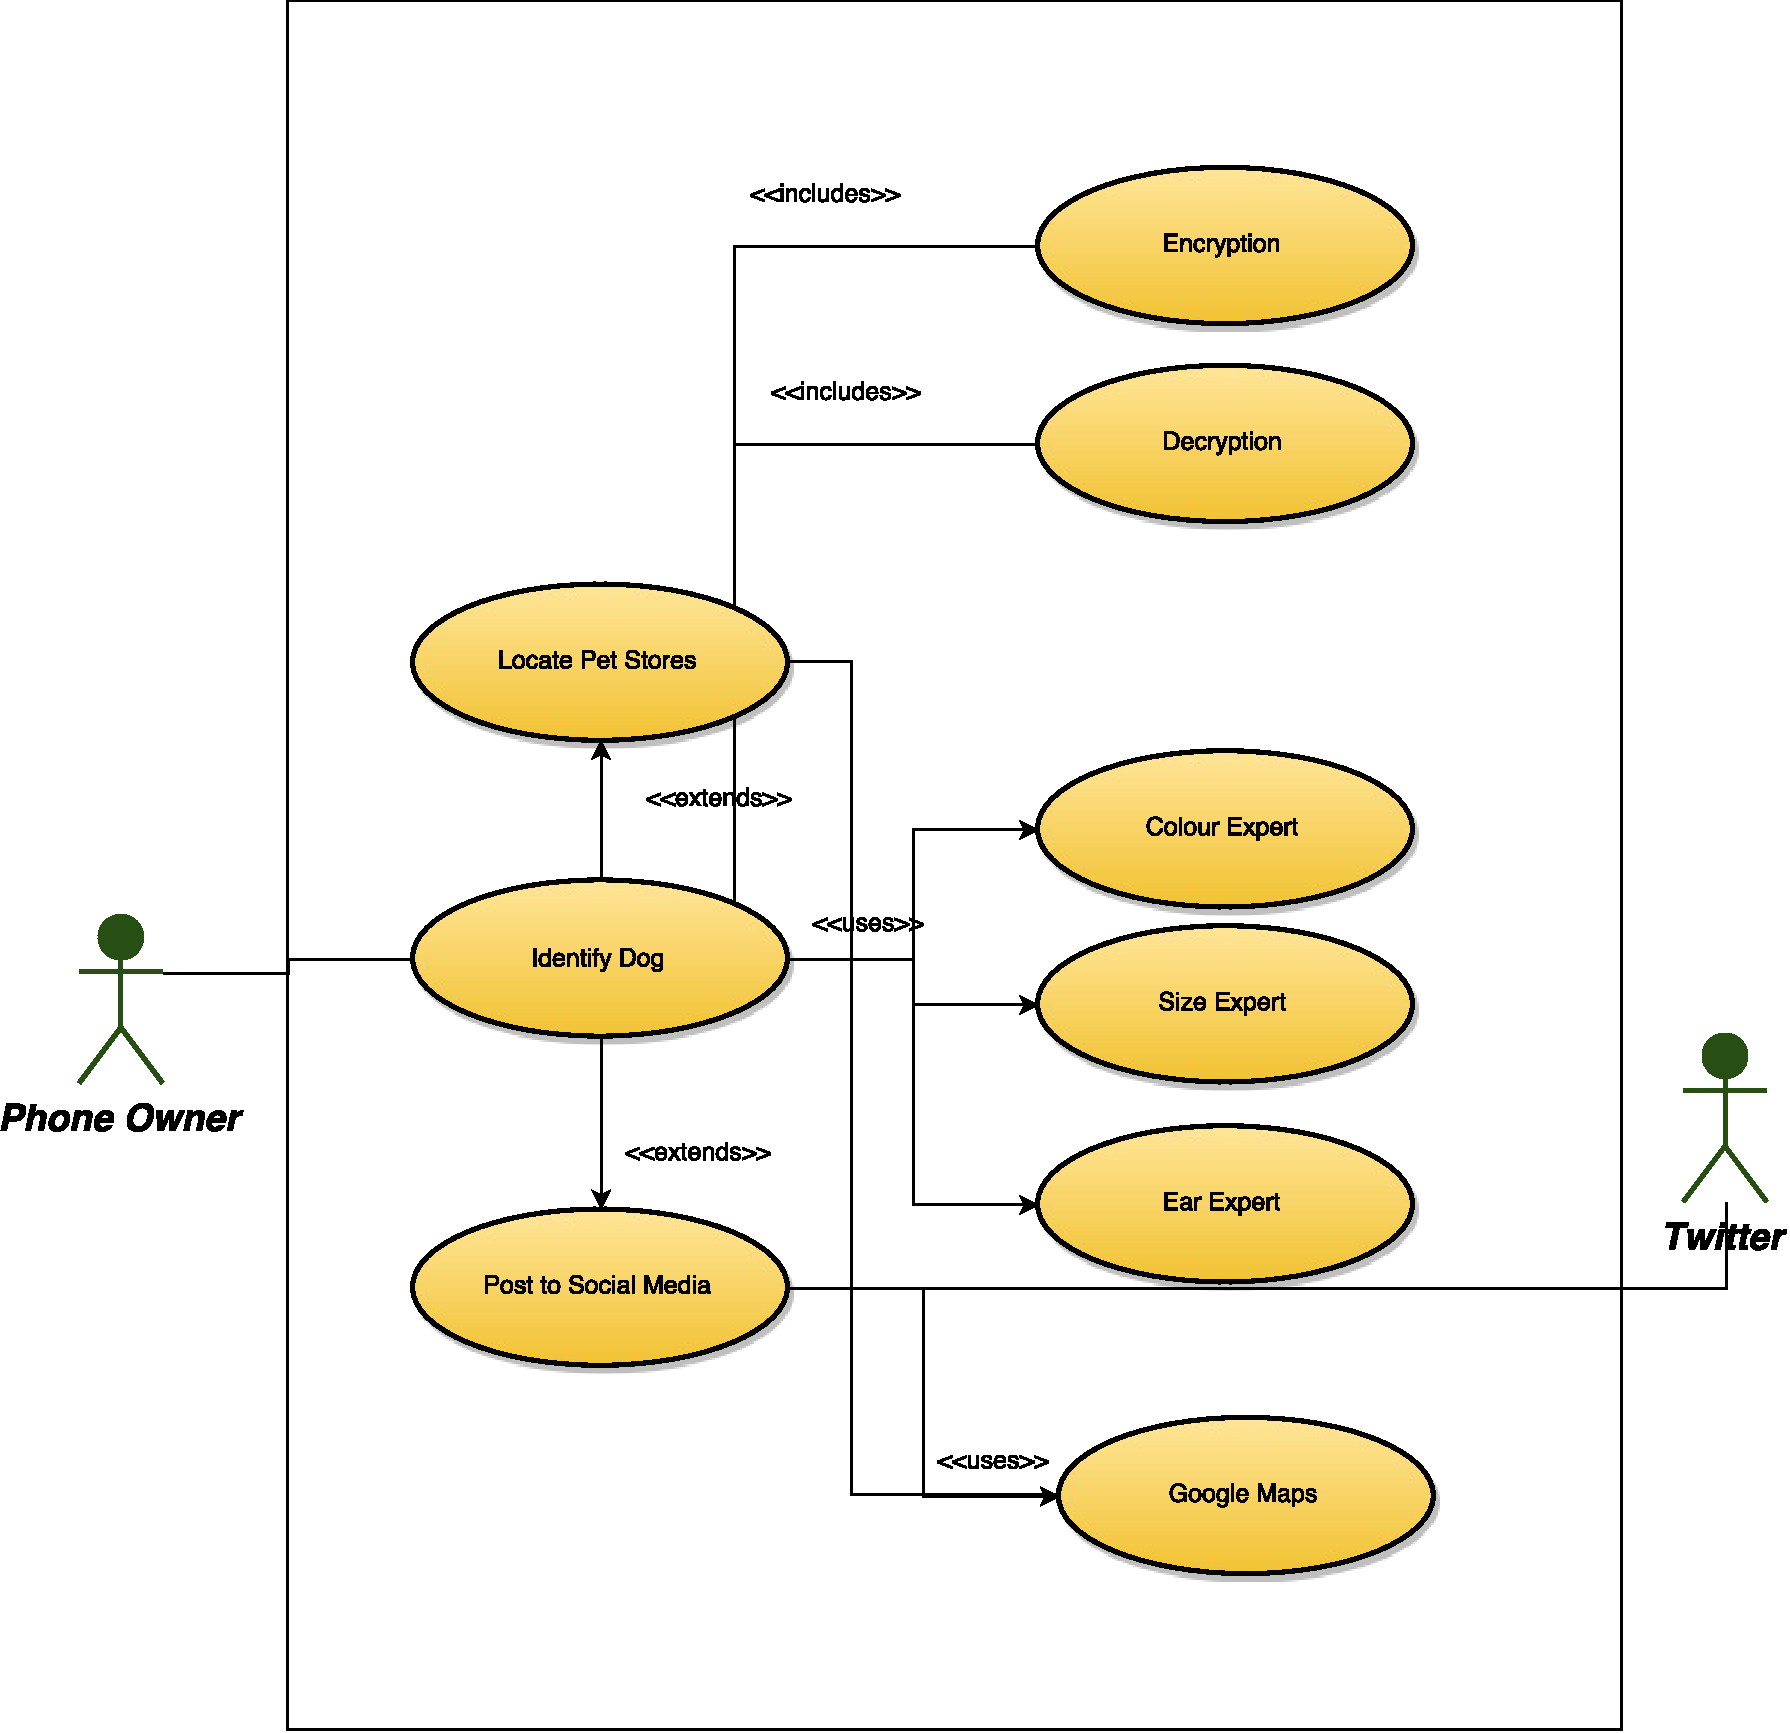
\includegraphics[width=\textwidth]{UseCase.pdf}
	\caption{\label{fig:analysisclassdiagram} A Use Case class diagram of the WhoDatDog system.}
\end{figure}

\begin{itemize}
	
	\item \textbf{Identify Dog} takes the user's description of the dog and attempts to identify the dog by using the experts associated with it.
	  
	\item \textbf{Locate pet stores} is an additional option after the system has identified the dog.  It should provide the user the locations of the nearest pet stores of the identified dog. 
	
	\item \textbf{Post to social media} is an additional option after the system has identified the dog. It should allow the user to post his results to twitter. 
	
	\item \textbf{The Colour Expert} determines the types of dogs that match with the user's colour description
	
	\item \textbf{Size Expert} determines the types of dogs that match with the user's size description
	
	\item\textbf{Ear Expert} determines the types of dogs that match the user's ear description
	
	\item \textbf{Google Maps} determines the location of the phone owner. 
	
	\item \textbf{Encryption} encrypts the data being passed around from class to class.
	
	\item \textbf{Decryption} decrypts the date being passed around from class to class. 
	

\end{itemize}




\section{Analysis Class Diagram}
\label{sec:analysisclassdiagram}

\begin{figure}[H]
\centering
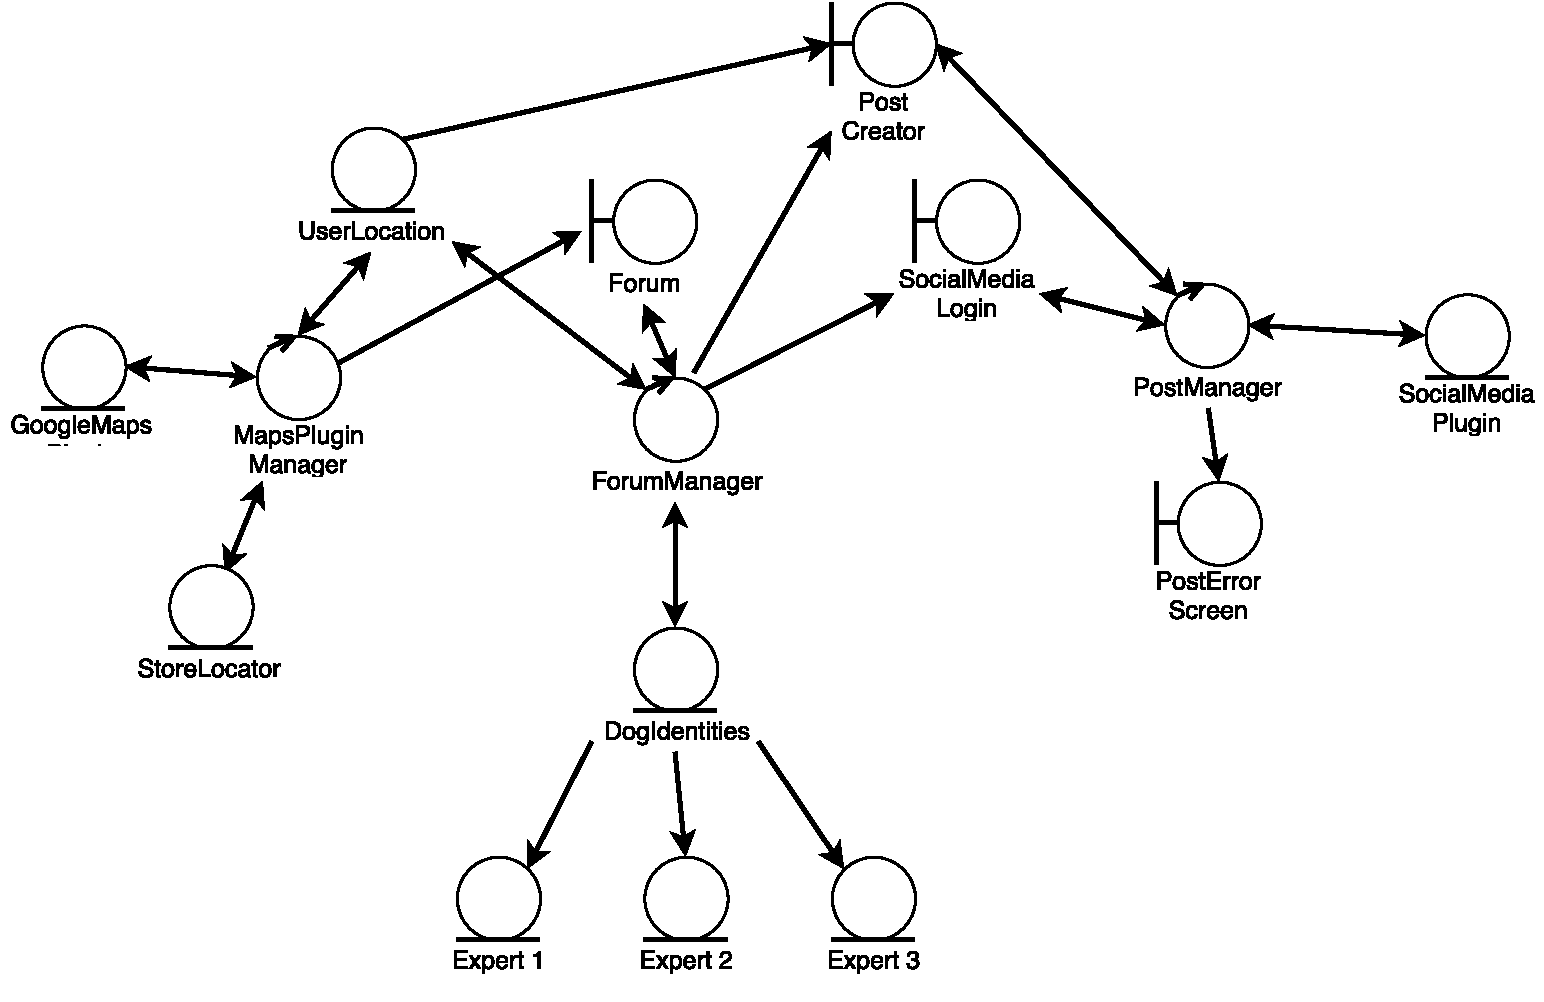
\includegraphics[width=\textwidth]{3A04_D2_Analysis_Class_Diagram.pdf}
\caption{\label{fig:analysisclassdiagram}An analysis class diagram of the WhoDatDog system.}
\end{figure}


\begin{itemize}
\item \textbf{Forum:} Boundary Class: Used as the main form of communication between the user and the system. Users can write text input to the forum, which the system will interpret and reply to.
\item \textbf{ForumManager:} Controller Class: Handles communication to and from the forum and the rest of the system.
\item \textbf{DogIdentities:} Entity Classes: Contains information regarding dog breeds. Connected to the three Expert entity sub-classes. This class receives a list of dog characteristics as input from the ForumManager class and returns a dog breed as input.
\item \textbf{Experts 1, 2 and 3:} Entity Classes: Each Expert contains information regarding a dog characteristic. When the DogIdentities class receives a request to identify a dog based on a list of characteristics, those characteristics are matched against those found in the Expert classes to determine the dog's breed.
\item \textbf{GoogleMaps:} Entity Class: Uses Google  Maps API Plugin as an entity from which geographical coordinates can be obtained.
\item \textbf{UserLocation:} Entity Class: Contains the user's current geographical location. Can optionally be used in the Post Creator class.
\item \textbf{StoreLocator:} Entity Class: Contains the geographical locations of pet stores, dog kennels, pounds, etc. locations near the user's own where the user may purchase/adopt a dog.
\item \textbf{MapsPluginManager:} Controller Class: Manages the interractions between the GoogleMaps, UserLocation, and StoreLocator classes. Can write responses to the Forum class regarding nearby stores.
\item \textbf{SocialMediaLogin:} Boundary Class: Prompts the user to enter their social media username and password.
\item \textbf{PostCreator:} Boundary Class: Used as a system interface through which the user can create a social media post. Also takes geographical information from the UserLocation class to use in the post.
\item \textbf{PostErrorScreen:} Boundary Class: Displayed if there is a communication error either with the social media post or the user's login credentials.
\item \textbf{SocialMediaPlugin:} Entity Class: A plugin for the Twitter social network service. Used as an entity class to access social network functionality such as the ability to create and publish posts.
\item \textbf{PostManager:} Controller Class: Manages the interractions between the PostCreator, SocialMediaLogin, PostErrorScreen, and SocialMediaPlugin classes.
\end{itemize}


% End Section

% End Section


\section{Architectural Design}
\label{sec:architectural_design}
% Begin Section

\subsection{System Architecture}
\label{sub:system_architecture}
% Begin SubSection

The overall architecture style that the WhoDatDog application will be using is the blackboard architecture style. This style seems to be the best suited towards our application because of the way our system is decomposed and how blackboard architecture relates to it. The blackboard architecture style is broken down into three parts:

\begin{enumerate}[1)]
	\item The blackboard: a sub-system used to store data (hypotheses and facts)
	\item The knowledge source: a sub-system (domain-specific knowledge is stored)
	\item The controller: a sub-system used to initiate the blackboard and knowledge sources
\end{enumerate}

These three sub-systems relate closely to the WhoDatDog application system. The blackboard being the inputs the user commits explaining what facts about the dog they are seeing, the knowledge source being the experts within the application with a controller of our own to allow the two to communicate with each other. The blackboard architecture style seems to fit perfectly within our system for the vision that we have as well as what we are trying to accomplish.

\begin{figure}[H]
	\centering
	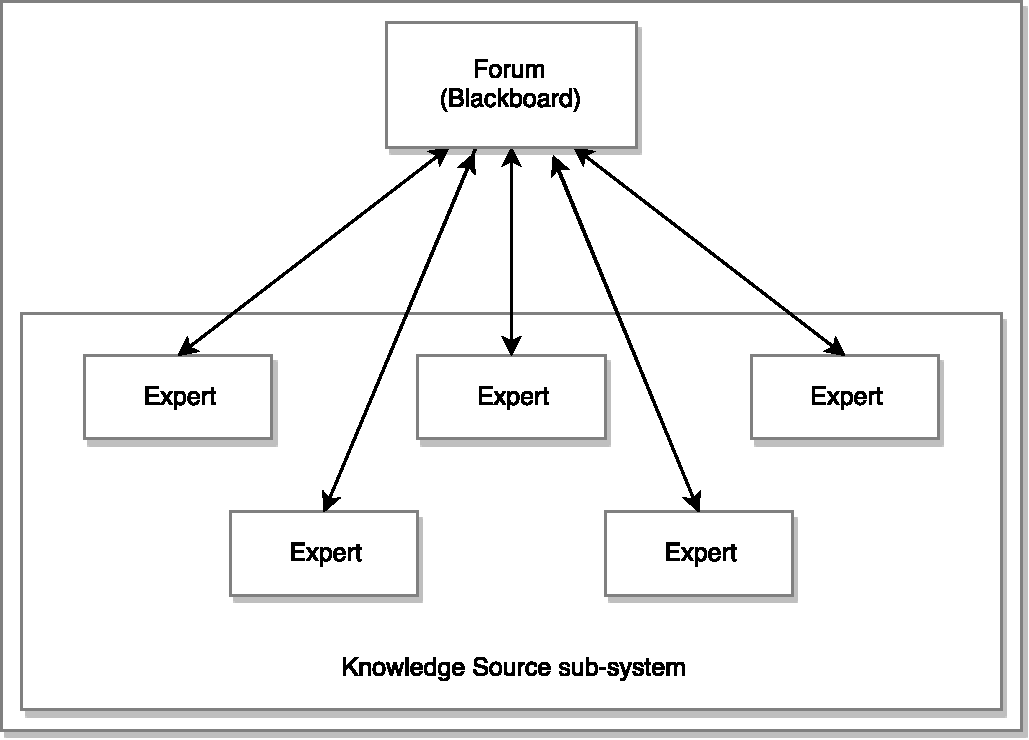
\includegraphics[width=\textwidth]{blackboardDiagram.pdf}
	\caption{\label{fig:blackboarddiagram} A blackboard diagram of the WhoDatDog system.}
\end{figure}

\subsection{Subsystems}
\label{sub:subsystems}
% Begin SubSection
\begin{itemize}
	\item Forum (blackboard): The forum is the blackboard sub-system within the WhoDatDog application. It is the main interaction that the user has within the the system. This is the area where the user will input the characteristics of the dog. The inputs by the user will then be inspected and then cross referenced with the Experts sub-system.
	\item Experts (knowledge source): The knowledge source sub-system within the WhoDatDog application is where each expert is contained. The experts contain information about certain characteristics of dogs and are able to identify the dog based on user inputs. The experts sub-system interacts with the forum and searches for matches between there database and the user inputs.
	
\end{itemize}
% End SubSection

% End Section

\section{Class Responsibility Collaboration (CRC) Cards}
\label{sec:class_responsibility_collaboration_crc_cards}
% Begin Section
\begin{table}[H]
	\centering
	\begin{tabular}{|p{7cm}|p{7cm}|}
		\hline 
		\multicolumn{2}{|l|}{\textbf{Class Name:} expert} \\
		\hline
		\textbf{Responsibility:} & \textbf{Collaborators:} \\
		\hline
		Receives encrypted description & forum, encrypt \\
		\hline
		Does a search on the database & database \\
		\hline
		Receives search results from the database & database \\
		\hline
		Sends encrypted results to the forum & encrypt, forum \\
		\hline
	\end{tabular}
\end{table}
\begin{table}[H]
	\centering
	\begin{tabular}{|p{7cm}|p{7cm}|}
		\hline 
		\multicolumn{2}{|l|}{\textbf{Class Name:} forum} \\
		\hline
		\textbf{Responsibility:} & \textbf{Collaborators:} \\
		\hline
		Displays the user interface along with a place to receive user descriptions & \\
		\hline
		Sends encrypted description to the experts & encrypt, expert \\
		\hline
		Receives encrypted results from the experts & expert \\
		\hline
		Decrypts the results and display them to the user & encrypt \\
		\hline
		Sends encrypted post request & encrypt, socialMedia \\
		\hline
		Displays and waits for user confirmation & socialMedia \\
		\hline
	\end{tabular}
\end{table}
\begin{table}[H]
	\centering
	\begin{tabular}{|p{7cm}|p{7cm}|}
		\hline 
		\multicolumn{2}{|l|}{\textbf{Class Name:} encrypt} \\
		\hline
		\textbf{Responsibility:} & \textbf{Collaborators:} \\
		\hline
		Encrypts user's description to the forum and sends back to the expert & forum, expert \\
		\hline
		Decrypts user's input in forum and send it back to the forum & forum \\
		\hline
		Encrypts social media post message when user confirms to post & forum, socialMedia, database \\
		\hline
		Decrypts social media post message before posting & forum, socialMedia, database \\
		\hline
	\end{tabular}
\end{table}
\begin{table}[H]
	\centering
	\begin{tabular}{|p{7cm}|p{7cm}|}
		\hline 
		\multicolumn{2}{|l|}{\textbf{Class Name:} socialMedia} \\
		\hline
		\textbf{Responsibility:} & \textbf{Collaborators:} \\
		\hline
		Posts message on facebook/twitter & database, encrypt \\
		\hline
		Sends request to user & forum \\
		\hline
		Displays Social Media icons on forum & forum \\
		\hline
	\end{tabular}
\end{table}
\begin{table}[H]
	\centering
	\begin{tabular}{|p{7cm}|p{7cm}|}
		\hline 
		\multicolumn{2}{|l|}{\textbf{Class Name:} locationIdentifier} \\
		\hline
		\textbf{Responsibility:} & \textbf{Collaborators:} \\
		\hline
		Identifies current location & Google Map API \\
		\hline
		Searches for nearby pet stores & Google Map API \\
		\hline
		Displays location information & Google Map API, forum, encrypt \\
		\hline
	\end{tabular}
\end{table}
% End Section

\appendix
\section{Division of Labour}
\label{sec:division_of_labour}

Jonathan Yu - Use Case Diagram \\
Samuel Jackson - Architectural Design \\Bill Chen and Fiona Hu - Class Responsibility Collaboration \\Nikita Jagora - Introduction and Analysis Class Diagram\\

\end{document}